\documentclass{beamer}
\usepackage{amsmath}


\begin{document}
\newcommand{\bmu}[1]{\underline{\boldsymbol{#1}}}

\begin{frame}
  \frametitle{Demand Equations and Parameters}
  Model parameters are in bold-underline.  $x$, $w_s$, and $w_n$ are
  the normalized income and prices: $Y/P_m$, $P_s/P_m$, and
  $P_n/P_m$.  $\alpha_j$ is the budget
  fraction of component $j$.
    \begin{align}
    Q_s &=
    \bmu{A_s}\left(w_s\right)^{e_{ss}}\left(w_n\right)^{e_{sn}}\left(x\right)^{h_s(x)}.\\
    Q_n &=
    \bmu{A_n}\left(w_s\right)^{e_{ns}}\left(w_n\right)^{e_{nn}}\left(x\right)^{h_n(x)}.
    \end{align}
    where
    \begin{align}
      e_{ij} &= \bmu{g_{ij}} - \alpha_j
      \frac{\partial}{\partial \ln x} \ln\left(x^{h_i(x)}\right).\\
      h_s(x) &= \bmu{\kappa}^{-\bmu{\lambda}}
      \left(\bmu{\kappa}x\right)^{\bmu{\lambda}/x}.\\
      h_n(Y) &= \frac{1}{2\bmu{\nu_1}}\left(x\right)^{2\bmu{\nu_1}/\left(1-x\right)}.
    \end{align}
\end{frame}

\begin{frame}
  \frametitle{Staple and Nonstaple Demand Income Dependence}
  \begin{center}
    \includegraphics[width=0.85\textwidth]{fig/yfuncs.eps}
  \end{center}
\end{frame}

\begin{frame}
  \frametitle{Additional notes on Parameters}
  \begin{itemize}
    \item We require $g_{ij} = \frac{\alpha_j}{\alpha_i}g_{ji}$, so there are only three $g$
      parameters, which we label $g_{ss}$, $g_{nn}$, and
      $g_{\text{cross}}$.
    \item This makes a total of 8 parameters:
      \begin{itemize}
      \item 2 scale factors.
      \item 3 quasi-elasticities ($g$ matrix elements).
      \item 2 staple income dependence parameters.
      \item 1 nonstaple income dependence parameter.
      \end{itemize}
    \item The $\nu_1$ parameter is the income elasticity of nonstaple
      foods at $x=1$, \emph{neglecting} the income dependence of the
      budget fractions, $\alpha$.
    \item The parameters in $h_s$ are not particularly intuitive, but
      they can be transformed to a more intuitive pair: $\mu_1$,
      $x_0$.  These represent respectively the income elasticity at
      $x=1$ (neglecting $\alpha$ dependence) and the income level at
      which elasticity switches from positive to negative.
  \end{itemize}
\end{frame}

\begin{frame}
  \frametitle{Likelihood Function and Monte Carlo}
  \begin{equation}
    L = \sum_i \frac{(Q_i - \hat{Q}_i)^2}{\sigma_i^2}
  \end{equation}
  For two sets of model parameters $\vec{p}_1$ and $\vec{p}_2$, the
  \emph{odds ratio} for the two parameter sets is
  \begin{equation}
    R_{12} = \exp\left(L_1 - L_2\right)
  \end{equation}
  So, a difference of 5 in $L$ indicates an odds ratio of about 150:1.
\end{frame}

\begin{frame}
  \frametitle{Monte Carlo Results (model v. 0.2)}
  This model version had all $\sigma_i = 1.0$ and the symmetry
  condition misspecified as $g_{sn} = g_{ns} = g_{\text{cross}}$.
  \begin{center}
    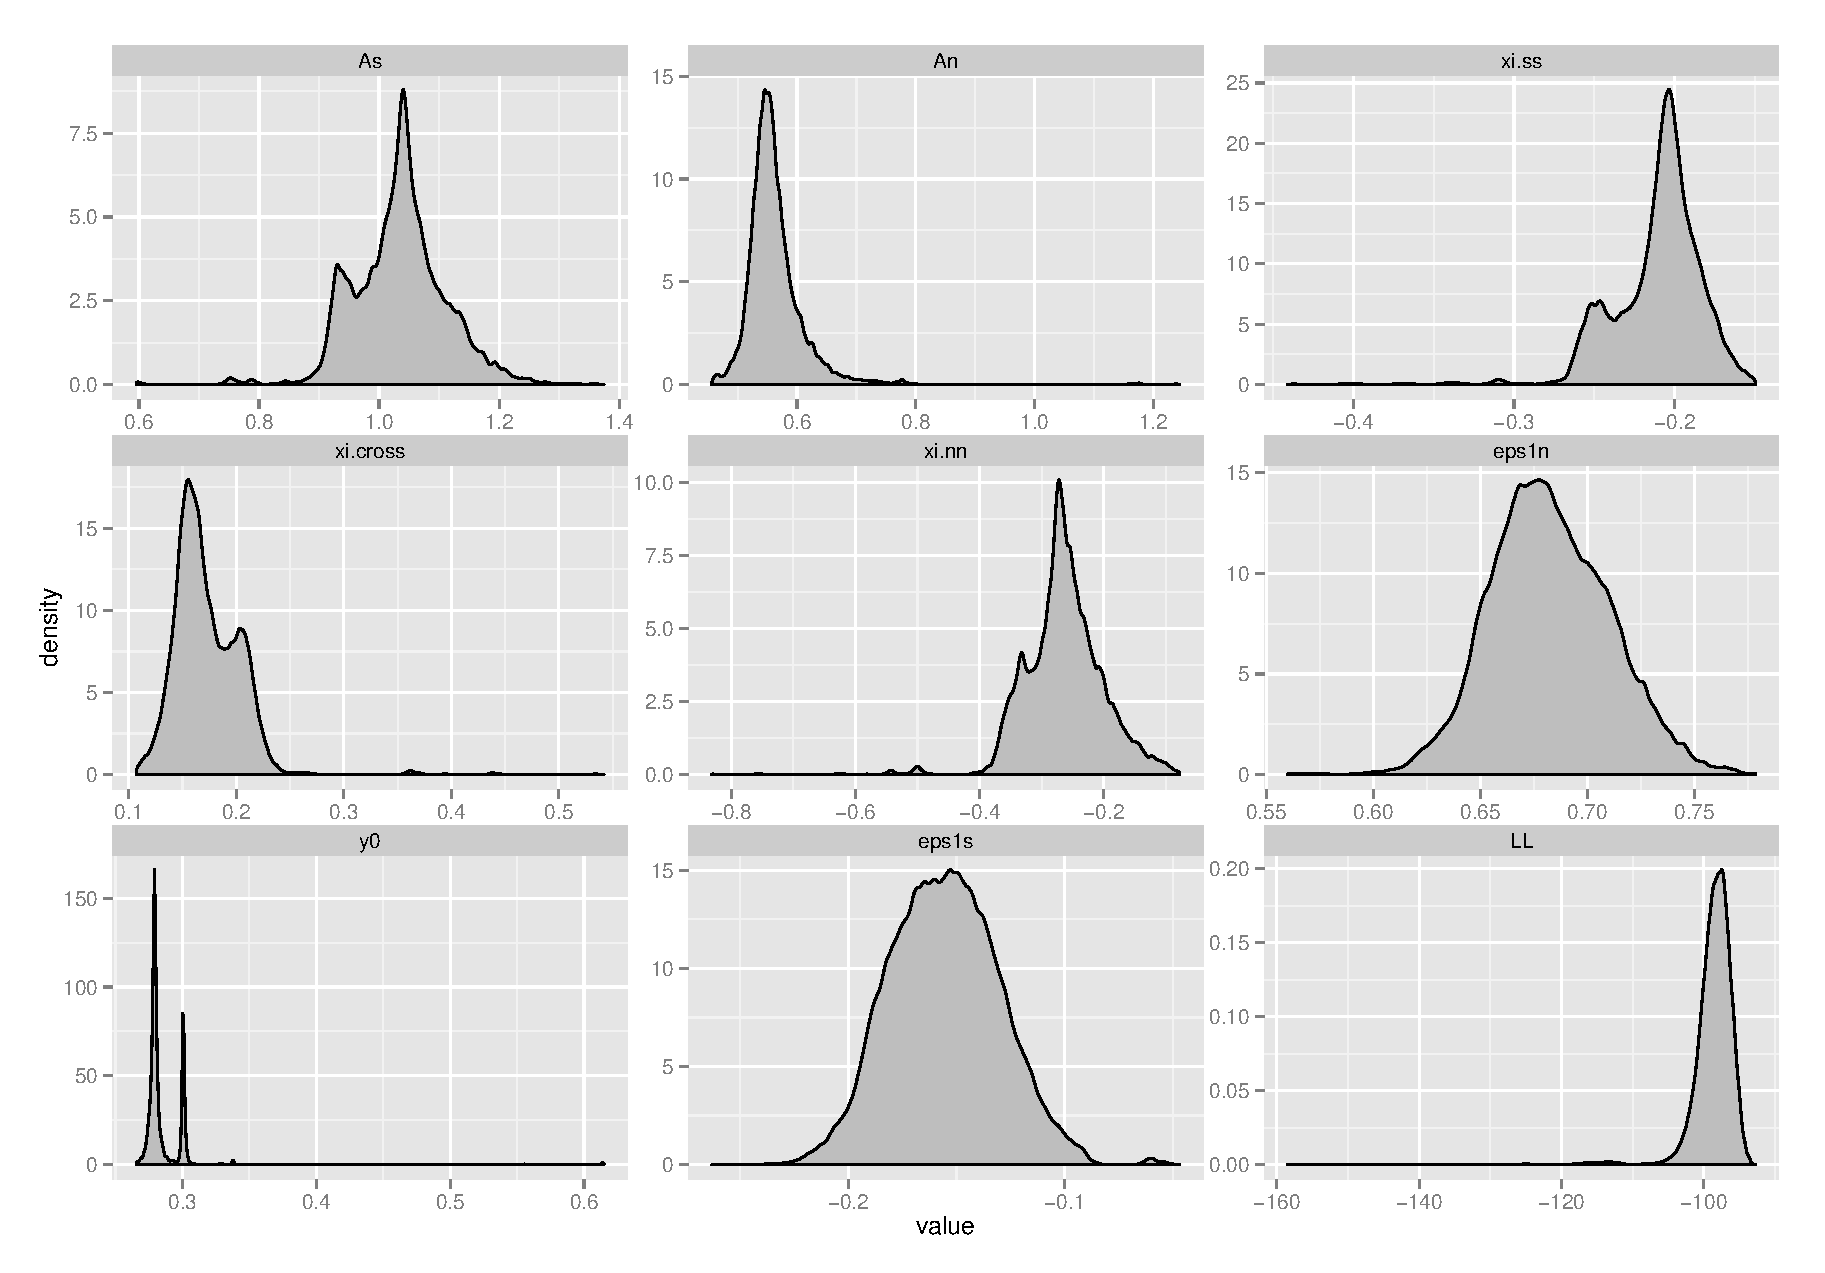
\includegraphics[width=0.85\textwidth]{fig/mcrslt-v0_2-allrgn.eps}
  \end{center}
\end{frame}

\begin{frame}
  \frametitle{Monte Carlo Results (model v. 0.4)}
  In this version we corrected the symmetry condition added
  more reasonable $\sigma$ values for the observational data.
  \begin{center}
    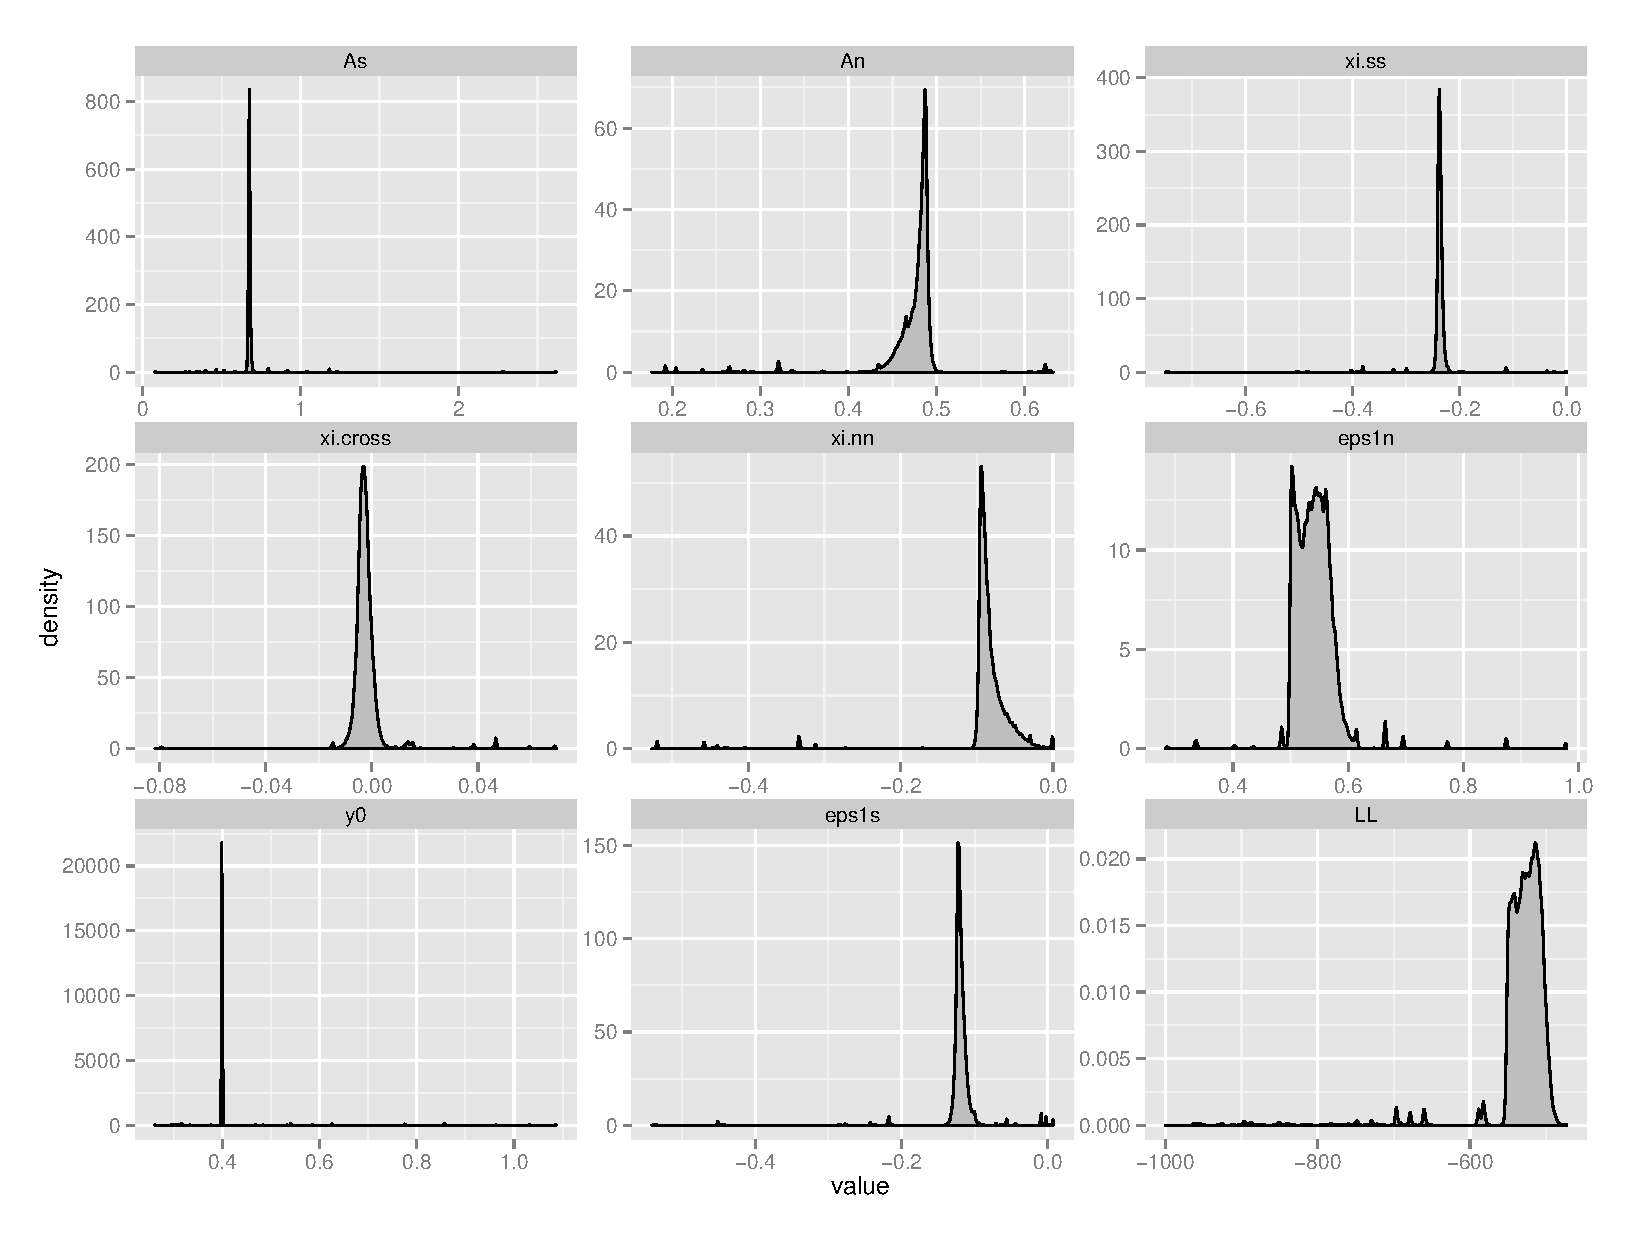
\includegraphics[width=0.85\textwidth]{fig/mcrslt-v0_4-allrgn.eps}
  \end{center}
\end{frame}

\begin{frame}
  \frametitle{Model Output (version 0.4)}
  \begin{center}
    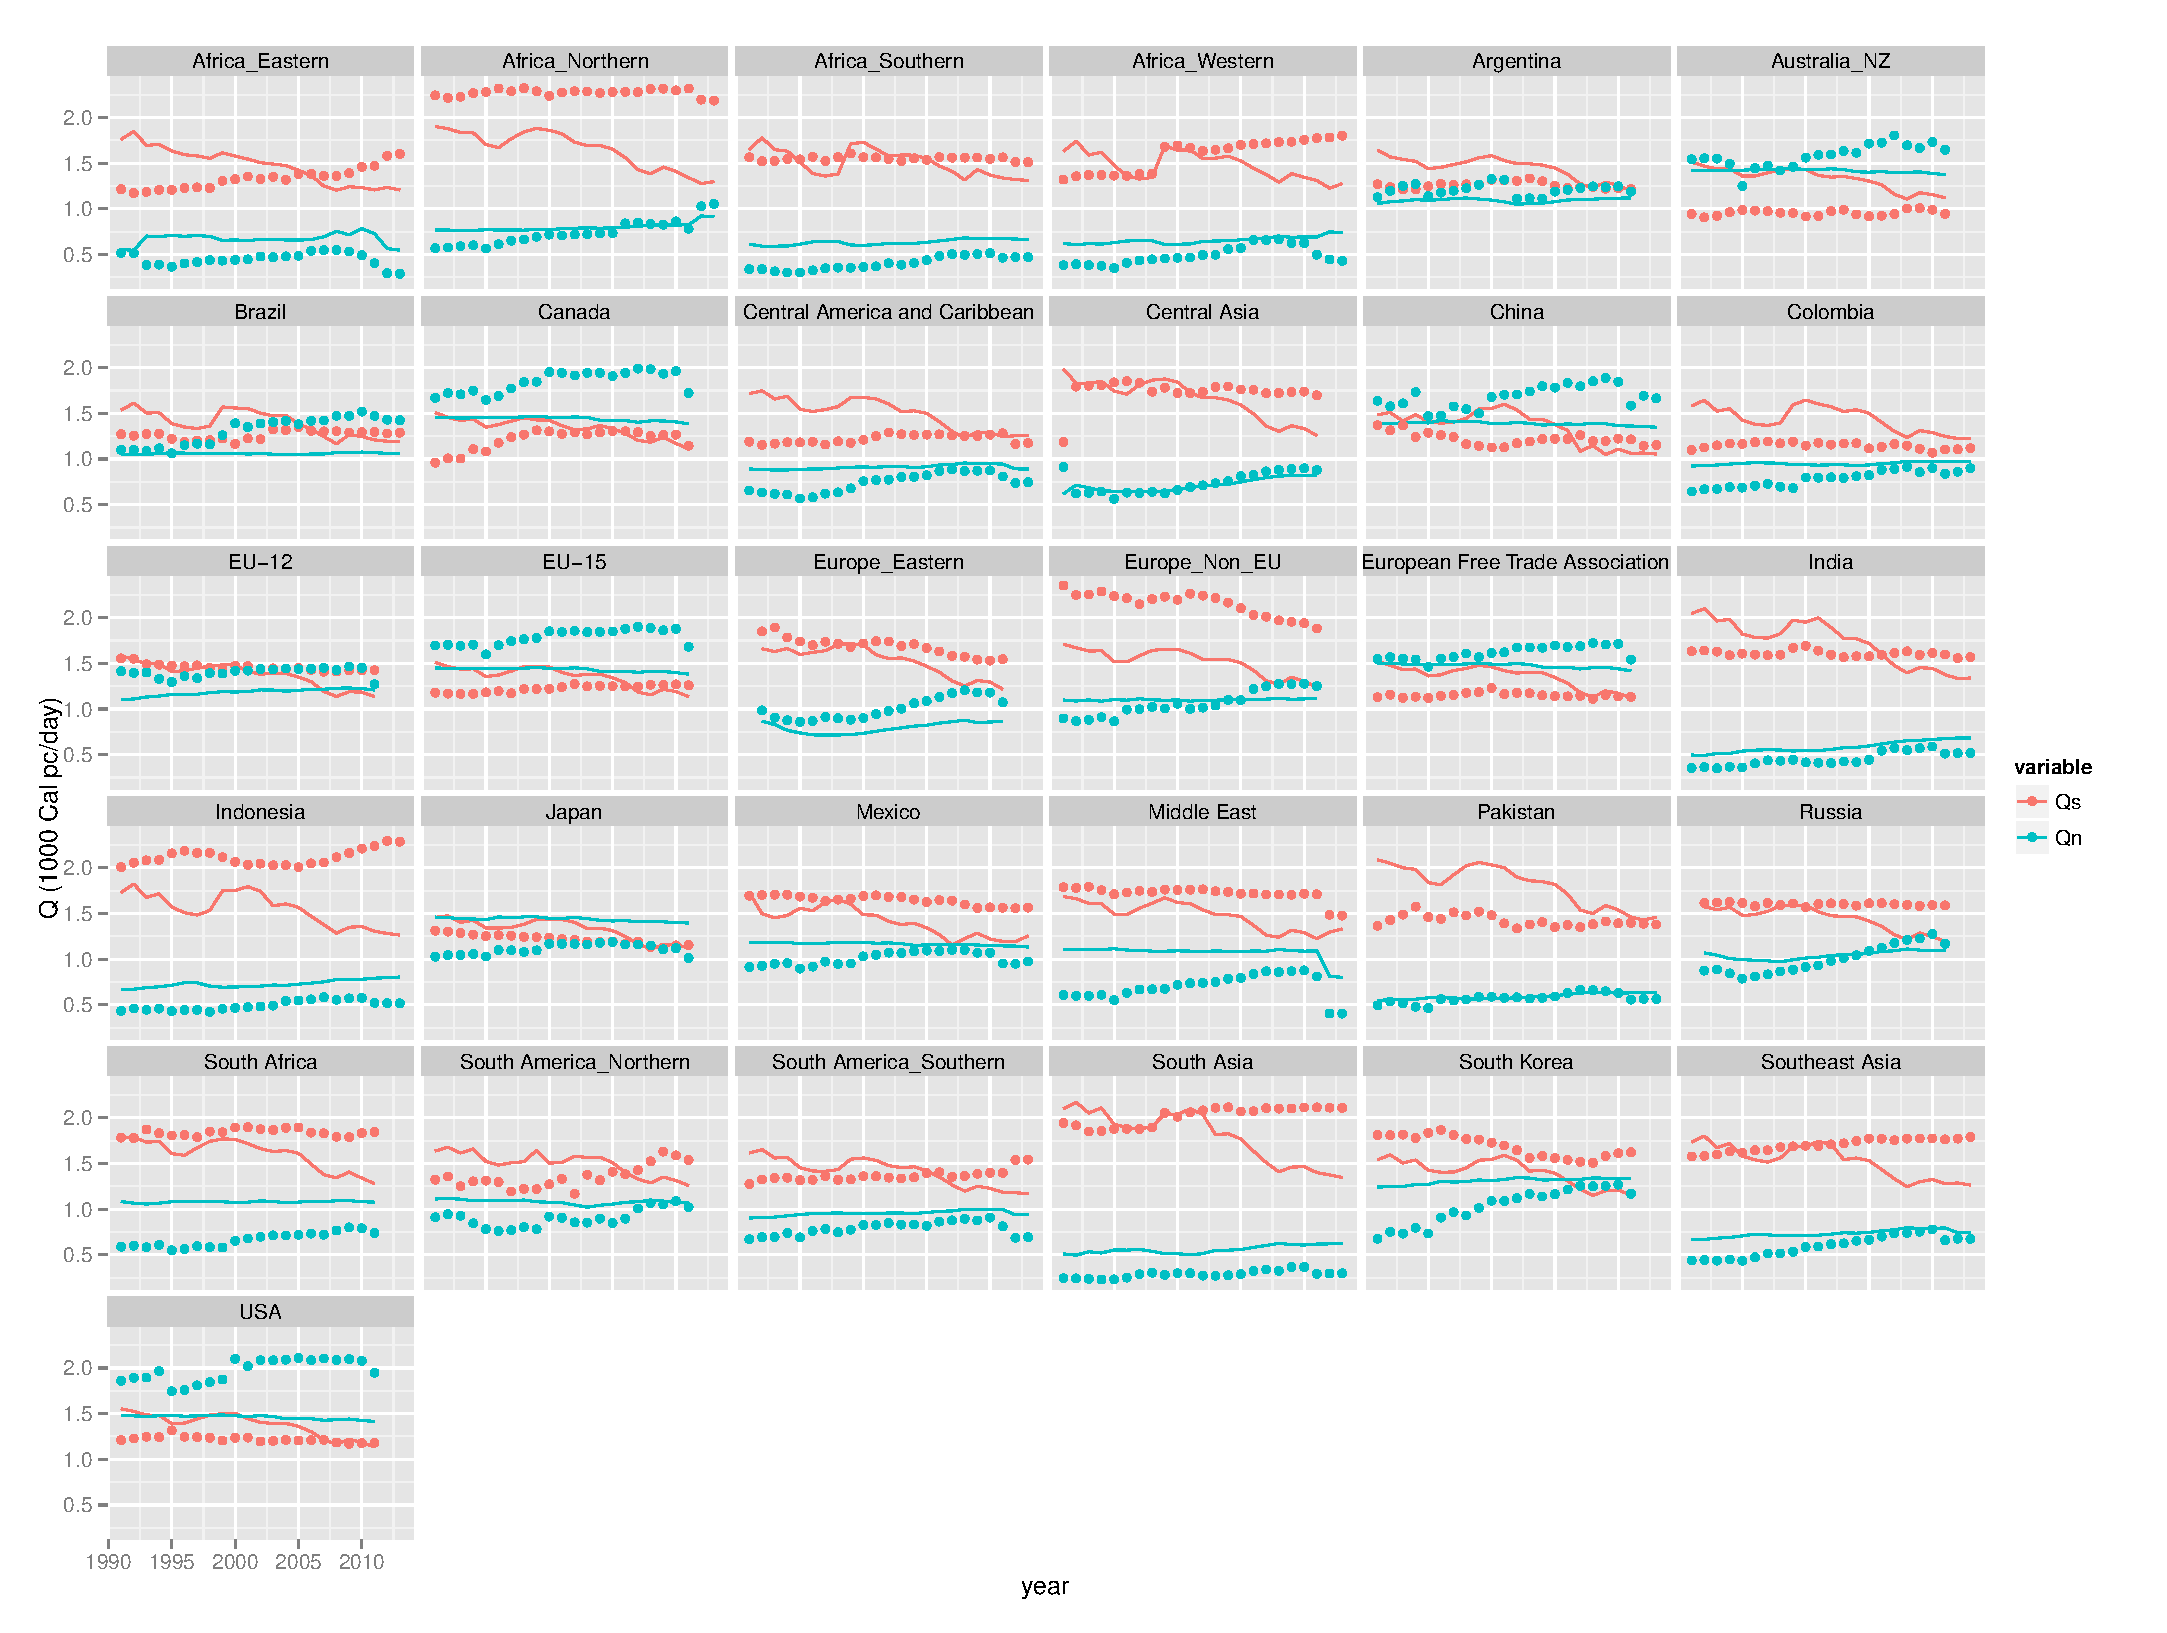
\includegraphics[width=0.85\textwidth]{fig/demand-byyear-allrgn.eps}
  \end{center}
\end{frame}

\end{document}
